\section{Methodology}
\label{s:methodology}
As mentioned in ~\autoref{s:related-work}, there are two challenges in cloaking
detection: reveal the content and handle dynamics of a webpage.

In order to model the dynamics of a webpage, we propose Simhash-based Website
Model, that is, use clusters learned from fuzzy hashs to model average and
variance of each change. This is based on the assumption that, the content and
layout of a website delivered to different users each time, is consistent
despite of the dynamic part on the page, e.g. advertisements. In order to reveal
the cloaked content, we design and implement simhash algorithm as browser
plugin, enabling crowdsourcing from user side.
Besides, we demonstrate the complexity of simhash algorithm, and show
that this plugin introduces negligible overhead to user browser.

\subsection{Simhash-based Website Model}
\label{ss:swm}
A website is usually rendered through Document
Object Model (DOM), which is maintained by browser in the fashion of a tree.
DOM tree contains information about layout of a website (Cascading Style
Sheets (CSS) is supplemental to DOM in describing the look and
formatting of a document). Out of various kinds of DOM nodes,  text nodes
represents the actual text that is displayed to user. This work focuses on
structure of DOM tree and text nodes that user actually sees, and use simhash
clusters to model them.

%Although, there are other interesting nodes, such as
%Javascript, we argue that Javascript need to modify the DOM tree to change what
%user actually sees, therefore, layout and text information suffices.

\subsubsection{Distance Approximation}
Simhash~\cite{charikar2002similarity} is a dimensionality reduction technique.
It is a fuzzy hash function family that maps a high dimension dataset into fixed
bits and preserves the following properties: 
(A) The fingerprint of a dataset is a "hash" of its features, and (B) The
hamming distance between two hash values is an estimation of the distance
between the original datasets.
This is different from 
cryptographic hash functions like SHA-1 or MD5, because they will hash two
documents which differs by single byte into two completely different hash-values and the
hamming distance between them is meaningless. 
In constrast, simhash will hash them into similar hash-values.

%However, simhash
%will hash them into similar hash-values (the Hamming distance would be small).
%In designing a near-duplicate detection system based on simhash, one has to deal
%with the quaintness of simhash de- scribed above. The strategy we employed is as
%follows: we design our algorithms assuming that Property A holds, i.e., the
%fingerprints are distributed uniformly at random, and we experimentally measure
%the impact of non-uniformity intro- duced by Property B on real datasets.


%Suppose P and Q are probability distributions over L, 
%\begin{multline}
%  EMD(P, Q) \le E[d(h(P), h(Q))] \\
%  \le O(\log{n}\log{\log{n}})EMD(P, Q).
%\end{multline}
%
%This equation is telling us that the hamming distance between simhash of set
%\b{P} and set \b{Q} is an approximation of Earth Moving Distance(EMD) between set P
%and Q. Charikar~\cite{charikar2002similarity} give the formal proof that the
%hamming distance of sets represents the cosine similarity.
%~\cite{manku2007detecting} implements an algorithm for creating text-based
%simhash for a website. In our work, we use the same simhash algorithm,

\subsubsection{Computation}
In terms of simhash computation, we use the same settings described in 
~\cite{manku2007detecting}, which turns out to be effective given the corpus of
8 billion websites over the Internet.

The computation of simhash start from a set of features.
Given a set of features extracted from a document and their corresponding
weights, we use simhash to generate an f-bit fingerprint as follows.
We maintain an f-dimensional vector V, each of whose dimensions is initialized to zero.
A feature is hashed into an f-bit hash value. These f bits (unique to the
feature) increment/decrement the f components of the vector by the weight of
that feature as follows: if the i-th bit of the hash value is 1, the i-th component
of V is incremented by the weight of that feature; if the i-th bit of the
hash value is 0, the i-th component of V is decremented by the weight of that
feature. When all features have been processed, some components of V are
positive while others are negative. The signs of components determine the
corresponding bits of the final fingerprint. In this work, we set f to 64.

\subsubsection{Requirements On Feature Set}
There are two characteristics in the computation of the simhash. First, the order of
the features doesn't matter because simhash is maintaining a global counter V.
Second, size of the feature set should be relatively large, because simhash is
random projection based approach, small set of features may result in completely
different simhash with one feature difference due to randomness.

The two characteristics can be considered as requirements in feature selection
phase: (A) If the order of feature matters, feature set should include
structural information. (B) Size of feature set should be relatively large.

%The order of the features in the original dataset does not matter, because
%the algorithm randomly projects each feature to f-dimensional vector and count
%the weighted presence in each dimension.
%(B) Size of the feature set should be relatively large. Simhash is known to
%perform badly on near duplicate detection when there are feature words. The
%reason is that, when the number of features are small, each feature votes too
%much on the vectors, difference in one feature may result in many bits of
%difference.
%
%Insight (A) is telling us, if the order of the original feature matters, the feature
%set should cover this. Insight (B) means, simhash works on relatively large
%number of datasets. The two insights are used in designing the text and dom
%simhash.

\subsubsection{Text Simhash and DOM Simhash}
%
%Charikar’s simhash [17] is a dimensionality reduction tech- nique. It maps
%high-dimensional vectors to small-sized fin- gerprints. It is applied to
%web-pages as follows: we first con- vert a web-page into a set of features, each
%feature tagged with its weight. Features are computed using standard IR
%techniques like tokenization, case folding, stop-word removal, stemming and
%phrase detection. A set of weighted features constitutes a high-dimensional
%vector, with one dimension per unique feature in all documents taken together.
%With simhash, we can transform such a high-dimensional vector into an f-bit
%fingerprint where f is small, say 64.
%
%
%In order to compress text information of a document, we extract the same set of
%text features as ~\cite{manku2007detecting}.
%
%Inspired from previous work, we understand that looking at only text would raise
%high false positive, therefore, we take into consideration the tag.
%
%In order to compress the structural 
%
%for compressing
%the text information. 
%

\begin{figure*}[t]
  \centering
  \subfigure[]{
    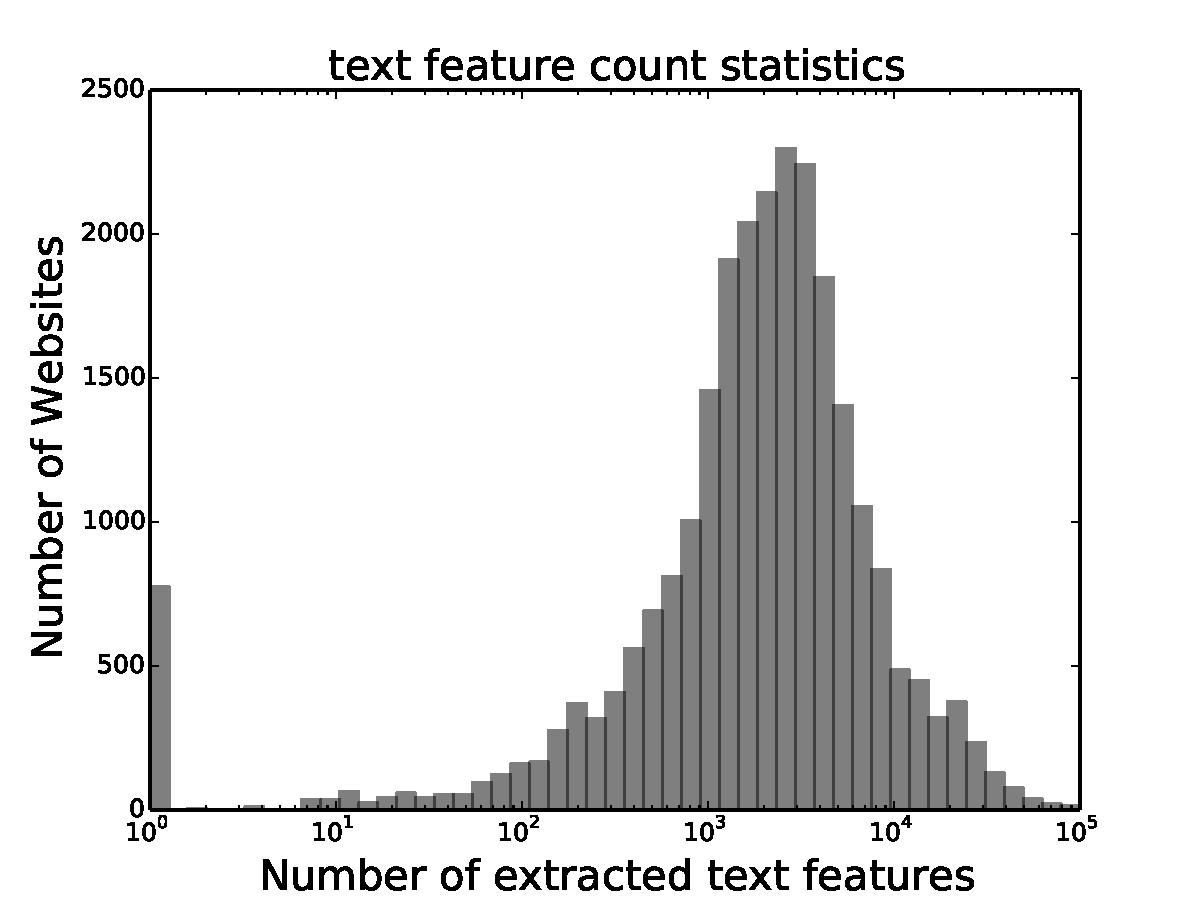
\includegraphics[width=.45\textwidth]{fig/text-feature-stats}
    \label{fig:text-feature-stats}
  }
  \subfigure[]{
    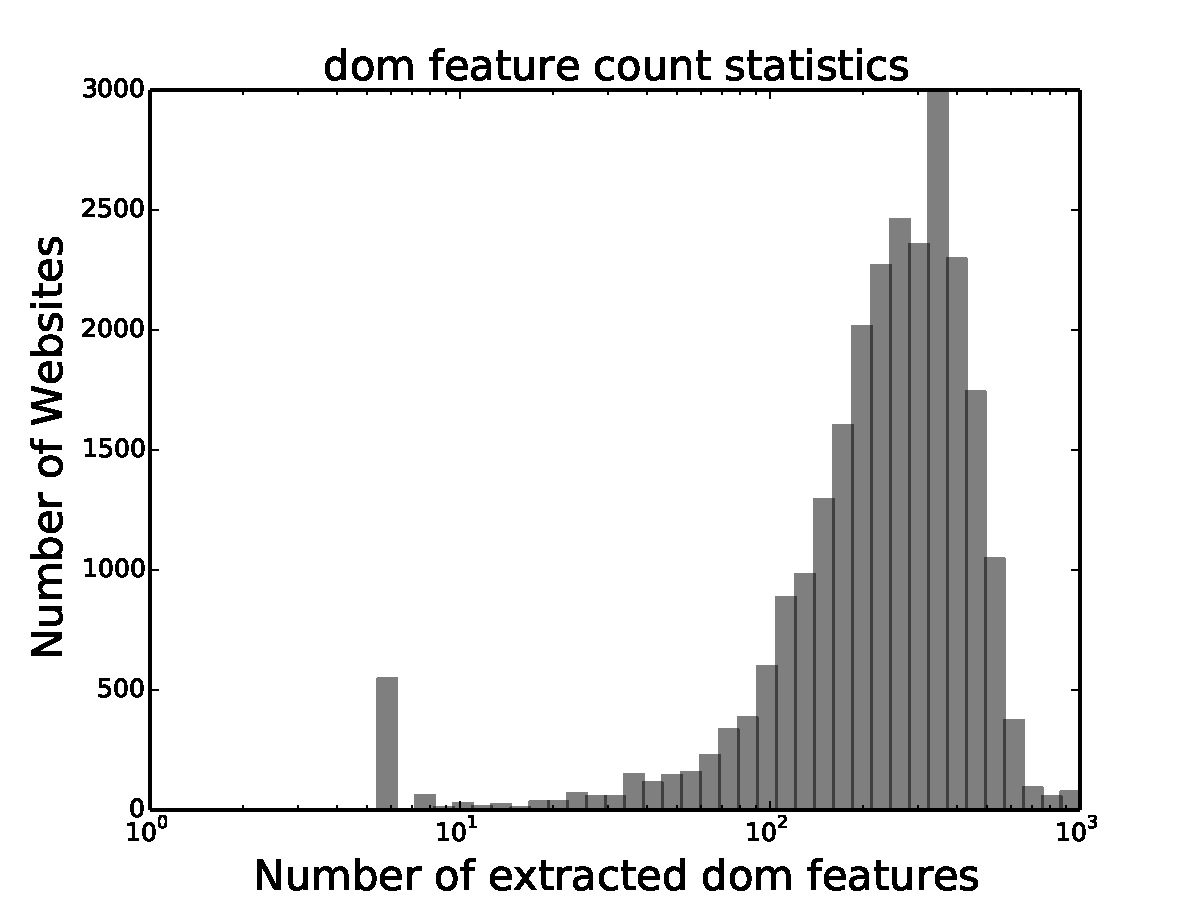
\includegraphics[width=.45\textwidth]{fig/dom-feature-stats}
    \label{fig:dom-feature-stats}
  }
  \caption{Number of text and DOM features extracted from different websites}
\end{figure*}

In order to detect cloaking, we need to capture the bahavior and similarity that
a same website maintains. Inspired by ~\cite{wang2011cloak}, this work looks at
both text and DOM features and generate simhash separately.
%We implemented the text-simhash algorithm 
%same as the simhash algorithm used in spam detection by Google.
%described
%in ~\cite{manku2007detecting},

For text simhahsh, the algorithm extracts visible sequence of words from website.
From the sequence, this algorithm extracts words, bi-gram, tri-gram set
(repeated elements only recorded once). For example, for
sentence: thank you so much, corresponds to feature set \{thank, you, so, much,
thank you, you so, so much, thank you so, you so much\}.
Because there are usually large number of words on a website, Requirement (B)
suffices. ~\autoref{fig:text-feature-stats} shows text feature statistics on %25610 urls in
urls obtained from hot search results $D_{hot, search}$. Since bi-gram, tri-gram 
shows how words are concatenated and represents strcture of documents,
Requirement (A) suffices. This algorithm is used rather than weighted version
described in  ~\cite{manku2007detecting}, because it is light-weight and doesn't
require inverse document frequency and phrase detection. This is important
in our case, because we are designing an algorithm that is deployable in user
browser, where efficiency matters.
%text feature set
%We implemented the text-simhash algorithm 
%same as the simhash algorithm used in spam detection by Google.
%described
%in ~\cite{manku2007detecting},

%and has great benefit in our use scenario, because this requires a single pass
%of the document and no extra information. In contrast,
%~\cite{manku2007detecting} implement extract weighted features using standard IR
%techniques like tokenization, case folding, stop-word removal, stemming and
%phrase detection, and may introduce more overhead and need extra knowledge.

\begin{figure}[t]
  \centering
  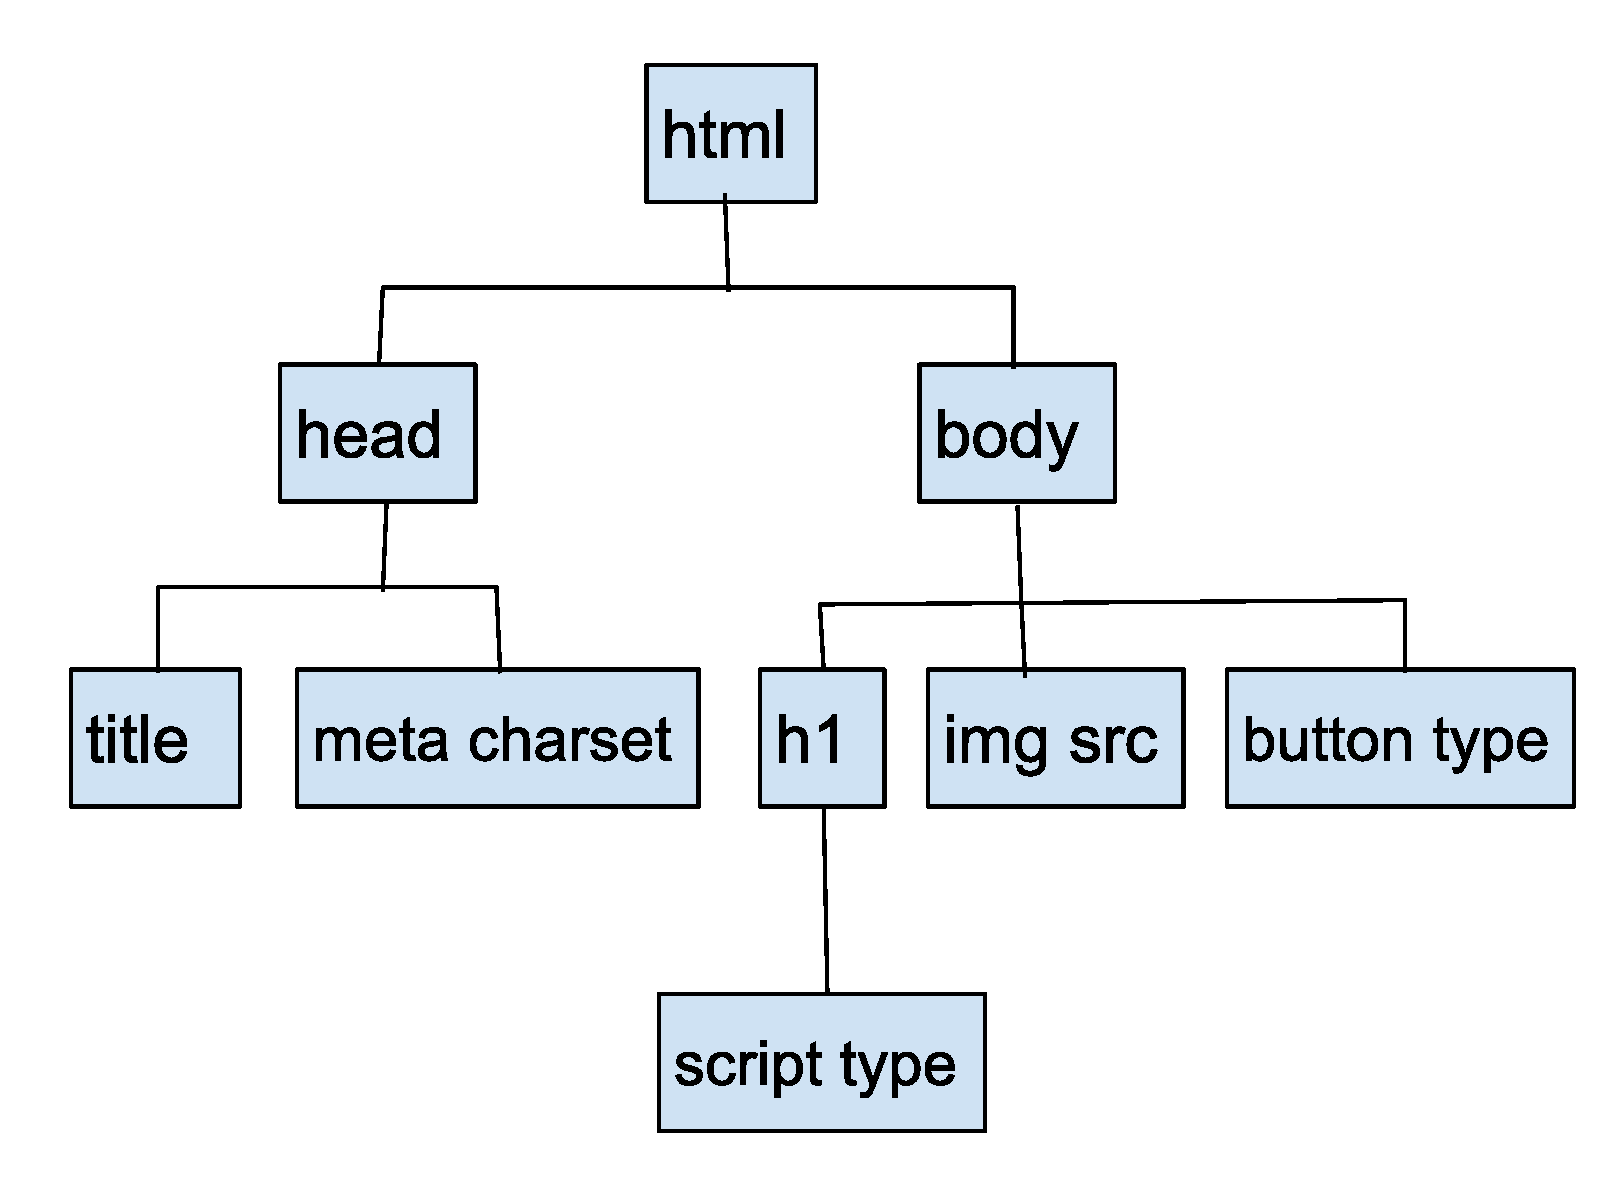
\includegraphics[width=.5\textwidth]{fig/dom-tree}
  \caption{DOM tree example}
  \label{fig:dom-tree}
\end{figure}

Regarding structure of websites, we design an algorithm to extract DOM features
out of DOM tree.

For each DOM tree, we record presence of each node (tag name), as
well as presence of each child parent pair. The node set tells us information about what
tag is present in this page, and child parent pair tells us how these tags are
organized, i.e., structure information, suffices Requirement (A).
Since we are recording presence of tags and type of tags are relatively small,
we record tag name and associated attribute names to gain more features (higher
entropy).
Attribute value is discarded because based on our observation, attribute value
may change on every visit.
For example,
~\autoref{fig:dom-tree} correspond to feature set 
\{html, head, body, title, \ldots, (head, html), (body, html), \ldots \}
%\{html, head, body, title,
%  meta charset, h1, img src, button type, script type, (head, html), (body,
%  html), (title, head), (meta charset, head), (h1, body), (img src, body),
%(button type, body), (script type, h1)\}

~\autoref{fig:dom-feature-stats} shows DOM feature statistics $D_{hot, search}$ and the number of features extracted in this
fashion is relatively large, suffices Requirement (B). 


% you can also use the wonderful epsfig package...
\begin{figure}[t]
  \centering
  \subfigure[User View of Yahoo Text Simhash]{
    \centering
    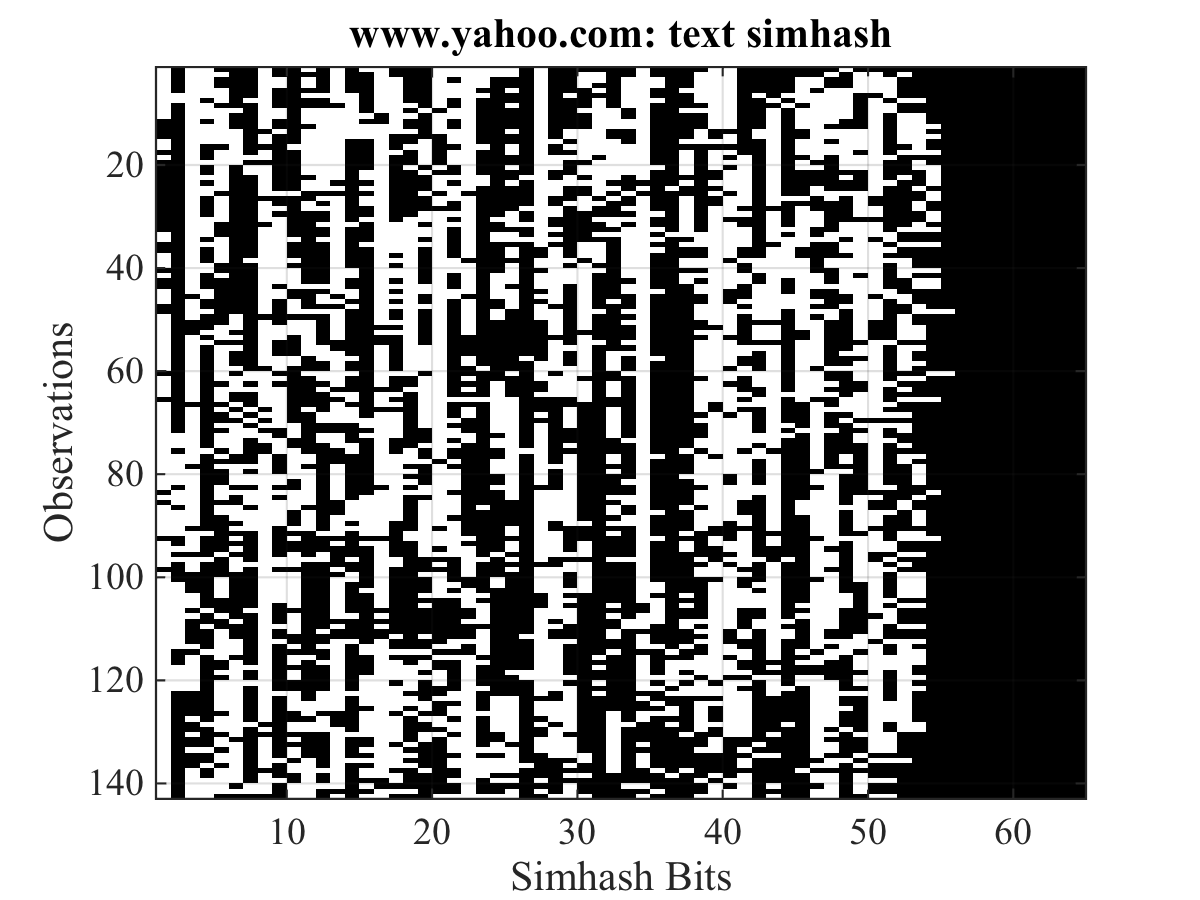
\includegraphics[width=.5\textwidth]{fig/yahoo-text-user}
    \label{fig:yahoo-text-user}
  }
  \subfigure[User View of Yahoo DOM Simhash]{
    \centering
    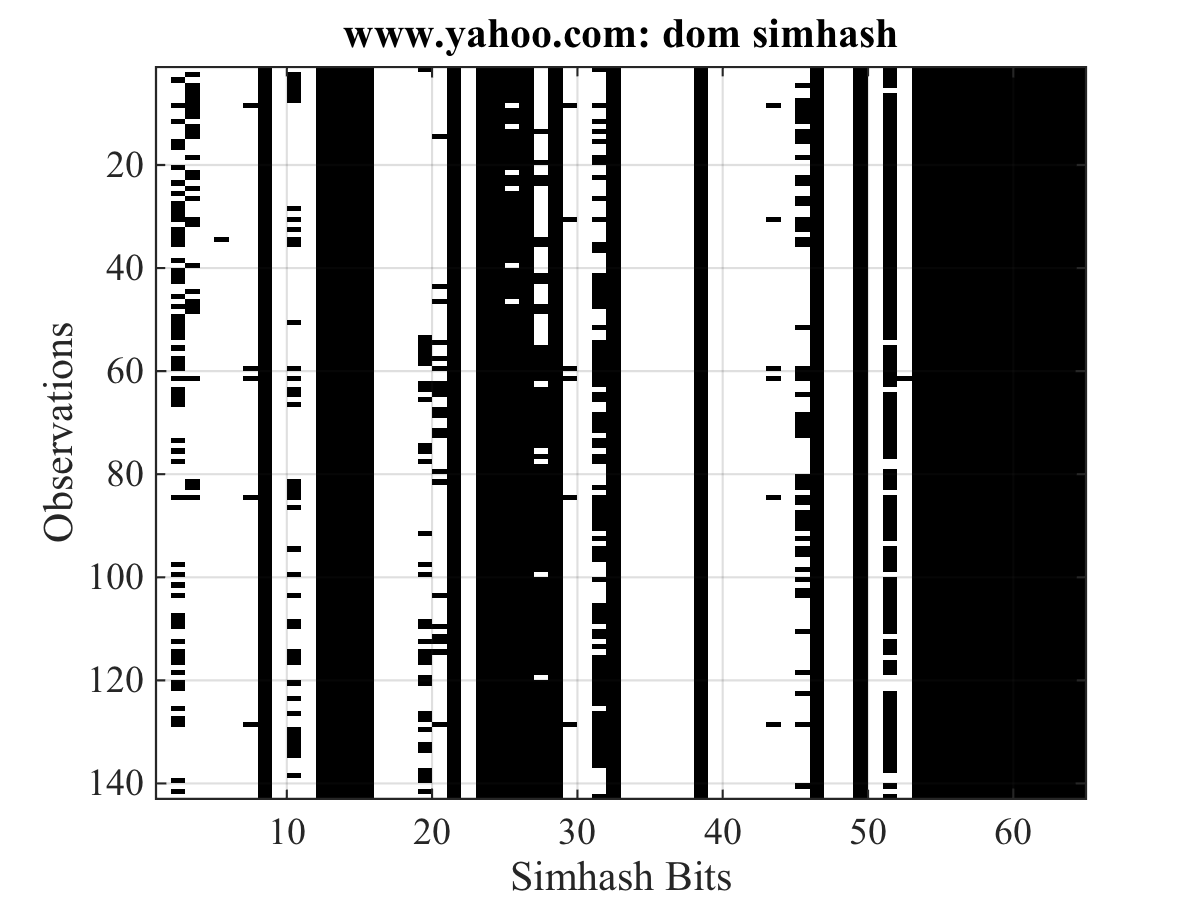
\includegraphics[width=.5\textwidth]{fig/yahoo-dom-user}
    \label{fig:yahoo-dom-user}
  }
  \caption{Yahoo simhash changes over 7x24 period Feb.1-7, 2015}
  \label{fig:yahoo-simhash}
\end{figure}

~\autoref{fig:yahoo-simhash} gives an example on how DOM and text simhash looks
like and how they are distributed on {\it www.yahoo.com} over 7 x 24 period from
Feb.1, 2015 to Feb.7, 2015. ~\autoref{fig:yahoo-text-user} shows text simhash
and ~\autoref{fig:yahoo-dom-user} shows DOM simhash. The x-axis is bits of simhash value and
y-axis is the id of each observation (id increases in the order of collection time).

It is pretty straightforward from ~\autoref{fig:yahoo-simhash} that,
text simhash changes rapidly, indicating dynamic nature of this
website, and DOM simhash changes relatively slow and less.

Till now, we have demonstrated the algorithm we are using to generate
text-simhash and DOM-simhash out of a website. Based on our observation, the
text-simhash might change rapidly, while DOM-simhash relatively remain the same.

\subsubsection{Clustering}
\label{sss:clustering}
Websites could have multiple versions of content due to many reasons.
An example is page construction. The server might return some notice or help
information for apology and instructions on what to do next.
Since we are monitoring websites over a period of time, we need to be able to
build model for different version of websites and learn corresponding pattern.

Different from ~\cite{manku2007detecting}, we not only want to know whether two pages are
duplicate, we also want to know the patterns of these simhash. In this work, we employ
hierarchical clustering to do this job.

Since simhash maps a high-dimensional
features set into fixed number of bits, where hamming distance represents the
similarity between the original feature set. We leverage the fact that hamming
distance is euclidean distance (L1 norm on 64 dimension). On each dimension, the
original value is either 0 or 1. But it can be averaged and centriod can be
computed.

In this work, we use agglomerative hierarchical clustering ~\cite{jones2014scipy} to cluster
collected simhash. This is a bottom up approach: each observation starts in its
own cluster, and pairs of clusters are merged as one moves up the hierarchy.
In order to decide which clusters should be combined, a measure of dissimilarity
between sets of observations is required. In most methods of hierarchical
clustering, this is achieved by use of an appropriate metric (a measure of
distance between pairs of observations), and a linkage criterion which specifies
the dissimilarity of sets as a function of the pairwise distances of
observations in the sets. This work represents each simhash as a 64 dimension
bit vector and specifies hamming distance as distance metric. The linkage method
used is average distance and criterion is inconsistent coefficient.

%These choices are reasonable. 
{\bf Average linkage:} 
Consider the following use case, spider collect
multiple copies of a website and compute corresponding simhash $S_{spider} = \{s_{i}, i \in
(1,n)\}$ and the user return observation $s_{user}$ for this website. In order to
compare $s_{user}$ with $S_{spider}$, and take into consideration of the all the
collected simhash, the distance from $s_{user}$ to centroid of $S_{spider}$ is a
reasonable measure. In order to be consistent with detection phase (user versus
spider), clustering phase uses average linkage as well.

{\bf Inconsistency coefficient:} this coefficient characterizes each link in a cluster tree by
comparing its height with the average height of neighboring links at the same
level and below it in the tree. The higher the value of this
coefficient, the less similar the
objects connected by the link. By using threshold of inconsistency
coefficient as criterion, we could get several clusters for each website.

\begin{equation}
  \label{coefficient:define}
  \alpha  = \frac{d - \mu}{\sigma}
\end{equation}

~\autoref{coefficient:define} explains how inconsistent coefficient is computed.
$\alpha$ is inconsistent coefficient, $d$ is the distance between two
clusters, $\mu$ is mean of the heights of all the links included in the
calculation, $\sigma$ is standard deviation of the heights of all the links
included in the calculation. In our case, each computation includes all links at
the same level and below it, and this is done by setting $depth$ in
$inconsistent(Z, depth)$ ~\cite{icintro} to $m-1$, where $m$ is total number of observations.


Let $T_{learn}$ denote the threshold for inconsistent coefficient, 
~\autoref{coefficient:learn} shows the merging criterion in clustering phase.
After clustering, $S_{spider}$ is divided into $c$ clusters $S_{spider, k}, k \in (1, c)$.
These clusters are Simhash-based Website Model for this website.

We denote each cluster $S_{spider, k}$ with centroid and links formed in
clustering phase $S_{spider, k} = \{centroid, links\}$. This representation is
intended for comparison with a new observation (single node cluster). $centroid$ is used to
compute distance from new observation to current cluster, $links$ are used
to compute $\mu$ and $\sigma$.

\begin{equation}
  \label{coefficient:learn}
  \begin{gathered}
    \alpha = \frac{d_{r,s} - \mu}{\sigma}, \text{merge } S_{spider, r},
    S_{spider, s} \text{ if } \alpha < T_{learn} \\
    \text{where }
    S_{spider, r} = \{s_{spider, r, i}, i \in (1, n_r), links_r\}, \\
    S_{spider, s} = \{s_{spider, s, j}, j \in (1, n_s), links_s\}, \\
    d_{r, s} = \frac{1}{n_rn_s}\sum_{i=1}^{n_r}\sum_{j=1}^{n_s} dist(s_{spider,
    r, i}, s_{spider, s, j}), \\ 
    \mu = avg(x), x \in  links_r \cup links_s, \\
    \sigma = std(x), x \in links_r \cup links_s \\
  \end{gathered}
\end{equation}

%For different websites, simhash can be considered as an algorithm to map them to
%a 64-bit number randomly ~\cite{manku2007detecting}. For the same website,
%simhash measures the similarity between them.
%



%In order to decide the number of clusters to take in hierarchical clustering
%(when to stop), we use inconsistent coefficient.
%
%considerations of significance, we ask whether this is an unusual result or
%whether it could have arisen merely by chance
%
%One way to determine the natural cluster divisions in a data set is to 
%linkage metric: hammming
%method: Unweighted average distance (UPGMA)
%cutoff: inconsistent value less than c
%pick inconsistent value now!!!!!
%


%\begin{gather*} \label{npa}
%  d(u,v) = \min(dist(u[i],v[j])) \\
%  \text{for all points i in cluster u and j in
%  cluster v. }
%\end{gather*}
%This~\autoref{npa} is known as the Nearest Point Algorithm.
%
%Single-linkage clustering is one of several methods of agglomerative
%hierarchical clustering. In the beginning of the process, each element is in a
%cluster of its own. The clusters are then sequentially combined into larger
%clusters, until all elements end up being in the same cluster. The stop
%criterion is the distance one.

\subsection{Cloaking Detection}
In the above section, for observations of each website, $S_{spider}$, we have 
learned clusters , which is $S_{spider, k}, k \in (1, c)$. For each cluster, we
represent it as $S_{spider, k} = \{centroid, links\}$.
In order to use these clusters, we first illustrate how the comparison can be
done.

In order to detect SEO and SEM cloaking,
this work first search and click results with normal user agent, then visit 
landing urls collected with google bot user agent (described in detail in
~\autoref{ss:dataset}).
For a specific website, we denote user observation of this website as
$s_{user}$, denote spider copies as $S_{spider}$ and 
$S_{spider, k}$ are the learned clusters.

For each cluster $S_{spider, k}$, we record link heights and centroid.
When comparing $s_{user}$ with $S_{spider, k} = \{centroid, links\}$, 
distance $d'$ from $s_{user}$ to $centroid$ is computed, which is average distance
from cluster $\{s_{user}\}$ to $S_{spider, k}$. In ~\autoref{sss:clustering}, we
merge clusters if inconsistent coefficient $\alpha < T_{learn}$. Similarly, we
could compute inconsistent coefficient $\alpha'$ for $\{s_{user}\}$ to $S_{spider, k}$ as
shown in ~\autoref{coefficient:detect} and use detection threshold to reject
$s_{user}$.

\begin{equation}
  \label{coefficient:detect}
  \begin{gathered}
    \text {If } \alpha' = \frac{d' - \mu}{\sigma} > T_{detect}, \text{reject } s_{user} \\
    \text{where }
    S_{user} = \{s_{user}\}, \\
   S_{spider, k} = \{centroid, links\}, \\
    d' = \frac{1}{n_k}\sum_{i=1}^{n_k} dist(s_{user}, s_{spider, k, i}) =
    dist(s_{user}, centroid), \\ 
    \mu = avg(x), x \in  \{d'\} \cup links, \\
    \sigma = std(x), x \in \{d'\} \cup links \\
  \end{gathered}
\end{equation}

For observation $s_{user}$, if all clusters $S_{spider, k}, k \in (1, c)$ rejects it, then
mark $s_{user}$ as cloaking.

\begin{figure}[t]
  \centering
  \subfigure[User View of Google DOM Simhash]{
    \centering
    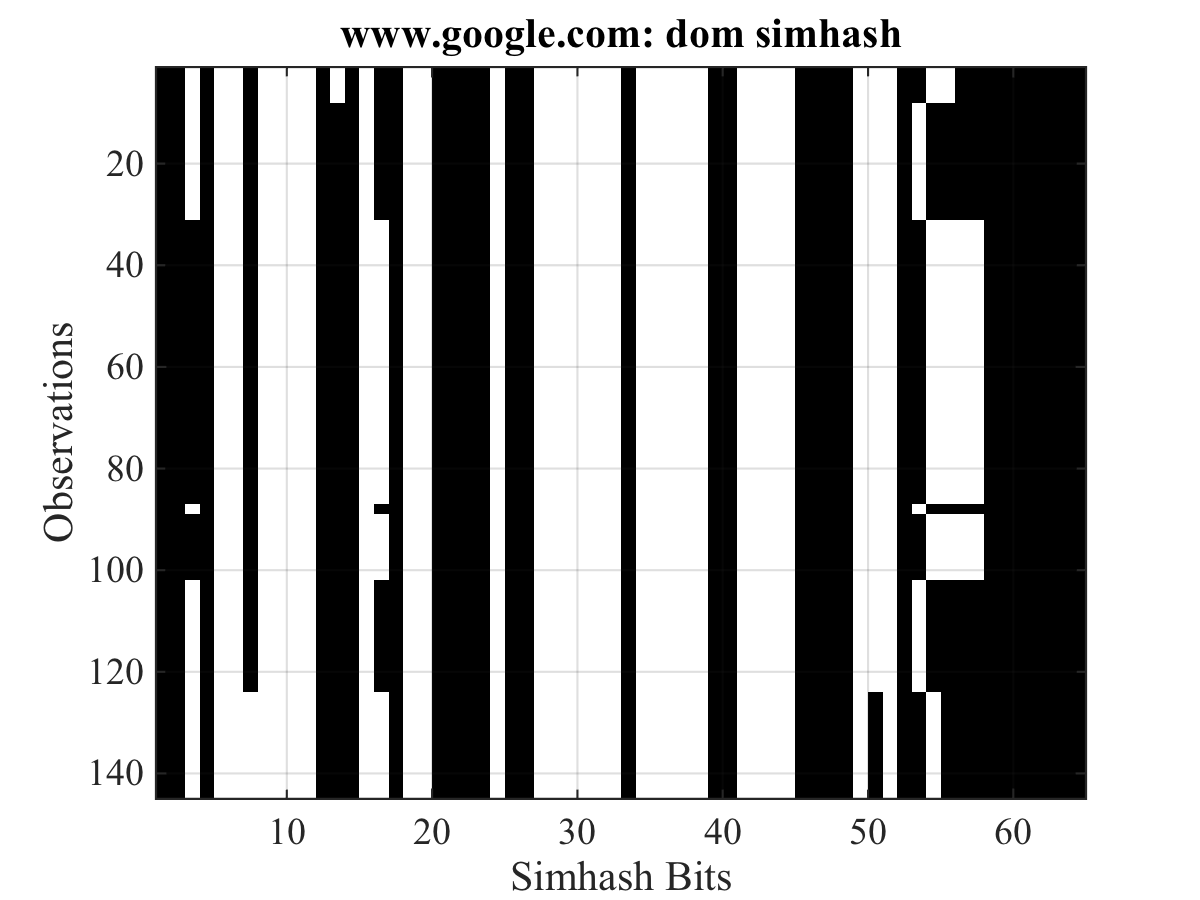
\includegraphics[width=.5\textwidth]{fig/google-dom-user}
    \label{fig:google-dom-user}
  }
  \subfigure[Spider View of Google DOM Simhash]{
    \centering
    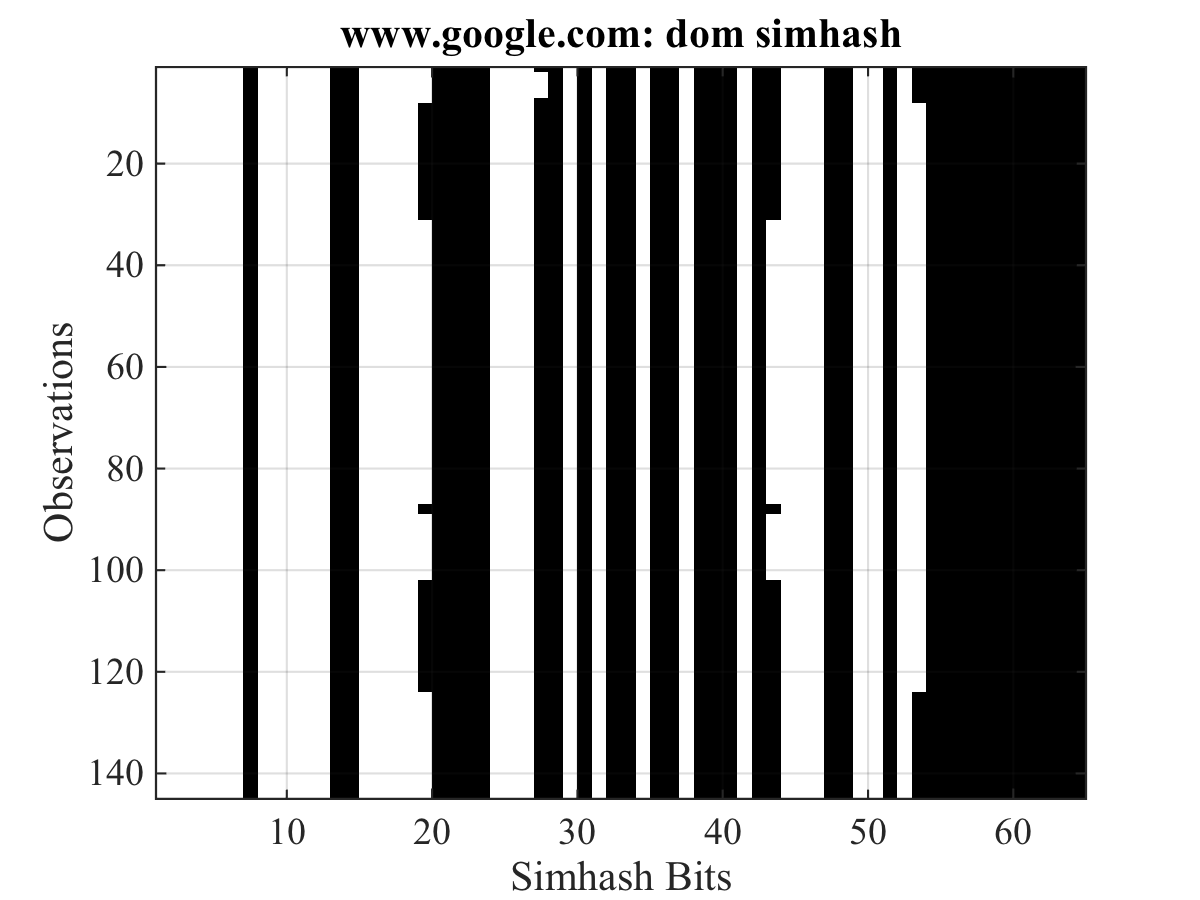
\includegraphics[width=.5\textwidth]{fig/google-dom-google}
    \label{fig:google-dom-google}
  }
  \caption{Comparison of user and spider copies DOM simhash, over 7x24 period Feb.1-7, 2015}
  \label{fig:google-simhash}
\end{figure}

However, in reality, there can be consistent differences between what spider
sees and what user sees and this is totally leagal. For example, a website
delivers non-javascript version to spider, but javascript version to user.
~\autoref{fig:google-simhash} shows the difference between spider and user
observations of {\it www.google.com} DOM simhash. Another example is that a website may
present advertisements to normal user, but non-advertisement version to spider.
Besides, there are websites that rarely changes at all, meaning $\sigma$ is
zero, thus ~\autoref{coefficient:detect} doesn't work. To fix the two problems, we introduce
a minimum radius $R_{detect}$. The modified formula is ~\autoref{radius:detect}:
\begin{equation}
  \label{radius:detect}
  \text{If } d' - R_{detect} - \mu > T_{detect} \sigma, \text{reject } s_{user}
\end{equation}

Next section ~\autoref{s:evaluation} evaluates the proposed SWM and cloaking detection
algorithm, and provides insights and suggestion on selection of $T_{learn}, T_{detect},
R_{detect}$.

%Classification hinges on having access to a robust set of features derived from
%URLs to discern between spam and non-spam. Previous work has shown that lexical
%properties of URLs, page content, and hosting properties of domains are all
%effective routes for classification [15], [16], [22]–[24]. We expand upon these
%ideas, adding our own sources of features collected by one of three components:
%a web browser, a DNS resolver, and IP address analysis. A comprehensive list of
%features and the component that collects them can be found in Table 1. A single
%monitor oversees multiple copies of each component to aggregate results and
%restart failed processes. In turn, the monitor and feature collection components
%are bundled into a crawling instance and replicated in the cloud


%\subsection{Model Selection}
%
%
%\begin{table*}[!th]                                                     
%  \centering                                                            
%  \scriptsize                                                           
%  \begin{tabular}{lllllllllll}
  \toprule
  & \multicolumn{2}{c}{\textbf{Normal}}
  & \multicolumn{2}{c}{\textbf{Lognormal}}
  & \multicolumn{2}{c}{\textbf{Exponential}}
  & \multicolumn{2}{c}{\textbf{Gamma}}
  & \multicolumn{2}{c}{\textbf{Logistic}}\\

  \textbf{Website(Hash Type)\textbackslash Model}
  & AD-value
  & P-value
  & AD-value
  & P-value
  & AD-value
  & P-value
  & AD-value
  & P-value
  & AD-value
  & P-value \\
  \midrule
  digg.com T & 0.617 &  0.100 & 0.481 &  0.219 &
  14.851 & < 0.003 & 0.538 &  0.186 & 0.531 &  0.131\\ 
  digg.com T & 0.227 &  0.806 & 0.179 &  0.914 &
  19.690 &  < 0.003 & 0.198 &  > 0.250 & 0.250 & >0.250\\
  yahoo.com T & 0.192 &  0.893 & 0.263 &  0.692 &
  35.828 & <0.003 &   0.231 & >0.250 & 0.222 & >0.250\\
  amazon.com T & 0.720 &  0.058 & 0.323 &  0.520 & 
  27.754 & <0.003 &  0.436 & >0.250 & 0.642 &  0.058\\
  reddit.com T & 0.373 &  0.411 & 0.331  & 0.509 & 
  35.063 & <0.003 & 0.340 & >0.250 & 0.361 & >0.250\\
  yacombinator.com T & 0.473 &  0.237 & 0.516 &  0.186 &
  37.551 & <0.003 & 0.519 &  0.204 & 0.583 &  0.089\\

  digg.com D & 0.319 &  0.372 & 0.348 &  0.305 &
  1.491 &  0.021 &  0.402 & >0.250 & 0.363 & >0.250\\
  yahoo.com D & 0.531 &  0.168 & 0.392 &  0.366 &
  18.837 & <0.003 & 0.441 & >0.250 & 0.584  & 0.088\\
  amazon.com D & 1.519 & <0.005 & 0.916 &  0.019 &
  22.083 & <0.003 & 1.052 &  0.009 & 0.548 &  0.114\\
  amazon.com D & 0.483 & 0.117 &  0.504 & 0.104 &
  1.741 & 0.010 & 0.601 & 0.128 & 0.523 & 0.115\\

\end{tabular}

                                     
%  \caption{Model statistics for selected websites}
%  \label{tbl:para-select}                                         
%\end{table*}                                                            
%
%
%This table ~\autoref{tbl:para-select} shows the Anderson-Darling (AD) value and P-value for each model.
%A common rule used in model selection is pick the model which has the smallest
%value with P-value greater than 5\%. Each row in the table represents one
%website. From the statistics of these websites, we choose normal distribution
%for text simhash and Lognomal distribution for dom simhash.
%
%In the simhash based cloaking detection model, input from the user is simply simhash. How to compare against the simhashs that is already collected?
%
%One simple way is to compute the average distance from this simhash to all the observed simhashs. The next step is then to tell whether this distance is reasonable. 
%
%The text distribution follows lognormal distribution.
%After mannual check of those results.
%
%

\subsection{Dataset}
\label{ss:dataset}
This work is focusing on detecting cloaking in SEO and SEM, therefore, we
collect search words for both SEO and SEM.

\subsubsection{Keywords}
Similar to ~\cite{wang2011cloak},
in order to detect and measure cloaking that intended to gather high volumes of
undifferentiated traffic, and those target on specific cloak search terms, we
collected two set of words, hot search words $W_{hot, search}$ and abuse
oriented words $W_{spam, search}$. $W_{hot, search}$ consists of 170
unique monthly hot search words
from Google trend ~\cite{google-trend} from Jan 2013 to Dec 2014. $W_{spam,
search}$ is first manually collected by referring to ~\cite{google-ad-policy} for
basic abuse oriented words in search engine, mainly from categories including
gaming ad network, adult-oriented content, alcoholic beverages,
dangerous products, dishonest behavior,
gambling-related content, healthcare and medicines. Then we expand $W_{spam,
search}$ using Google Suggest, and get 1024 words.

For SEM cloaking detection, the selection of keywords is a different, because
Google Adwords system is based on a real time bidding system and advertisers will bid on
monetizable keywords, e.g. instant loan, but not on navigational keywords, e.g.
facebook. Inspired from ~\cite{chellapilla2006improving}, we
collect monetizable words for advertisement collection. Monetizability is
measured by Google Keyword Planner (GKP) ~\cite{keyword-planner}. Keyword planner
provides convenient API for checking competition and suggested bid for list of
keywords. Similar to SEO, we collect monetizable keywords from hot search and
abuse oriented list. Abuse oriented ad words are collected by filtering words
that has no competition and no bid price in $W_{spam, search}$, as a result, 573
words composes spammy advertisement word set $W_{spam, ad}$. In order to get as
much advertisements as possible, we collect 11671 hot keywords from Google Trend
~\cite{google-trend} (from 2004 to 2014, and each categories are collected), 
filter this word set by GKP, and get 4108 keywords, $W_{hot, ad}$.

%9 cat: 686
%dishonest: 103
%
%gambling: 128
%dangerous: 64
%health: 43


%We have collected four datasets, spammy search, $D_{spam, search}$, hot search,
%$D_{hot, search}$, spammy ads $D_{spam, ad}$, hot ads, $D_{hot, ad}$. 
%$D_{spam, search}$, spammy search words collected manually, \XXX{N} words.
%$D_{hot, search}$, hot search monthly words from Jan 2013, Dec, 2014, 24 month
%in total,  \XXX{N} words.
%From $D_{hot, search}$, we evaluate the monetizability of each word through
%Google Keyword Planner~\cite{keyword-planner} and simply
%remove the words that have no bid price. This results in our spammy
%advertisements words set, $D_{spam, ad}$, we have collected advertisements from 573 words.
%$D_{hot, ad}$, we need as much words as possible, i.e. as much ads as possible,
%therefore first download hots words list from Google Trend, for hot words in
%each category, we download weekly, monthly, and yearly from 2004 to 2014, and
%then we find the useful keywords with Keyword Planner~\cite{keyword-planner}.
%We have collected advertisements from 4108 words.
%

%
%Because we want to measure cloaking in SEO and SEM, we have compiled a list of
%cloaking words, from the policies specified by Adwords, inspired by the words
%collection process in ~\cite{wang2011cloak}. We have looked at the policies, and
%collected \XXX{N} words, from ad network abuse, adult abuse, alcohol abusive, dangerous behavior
%abuse, dishonest behavior abuse, health abuse, gambling abuse.
%

\subsubsection{Crawling}
\label{sss:crawling}
Starting from the four collected keyword set, we automate browser to do
search-and-click. This work uses Selenium ~\cite{selenium}, an open source
browser automation tool, to visit websites while mimicked as users and spiders.
For SEO keywords crawling, we set browser user agent to 

{\it Googlebot/2.1
(+http://www.google.com/bot.html)}

to mimic Google bot and 

{\it Mozilla/5.0 (Windows NT 6.3; Win64; x64) AppleWebKit/537.36 (KHTML, like
Gecko) Chrome/37.0.2049.0 Safari/537.36}

to mimic Chrome user on windows
machine. For SEM keywords, Chrome user setting is the same, but spider user
agent is set to {\it AdsBot-Google (+http://www.google.com/adsbot.html)}, which
is the user agent used by Google to inspect ads and advertisement landing pages
are required by Adwords Policy ~\cite{google-ad-policy} to show consistent 
content to Google and normal user.

In SEO, we use a university IP running ubuntu to perform crawling (browser user
agent can be forged, thus will be considered as windows machine by site owner).
Since redirection is popular on Internet, what user actually clicks may not be
where he goes to. In this work, we denote the link that user directly clicks on
or input to browser as $URL_{visit}$, and resulting page that user is finally
led to as $URL_{landing}$.
The crawling process is: 
(A) For each word in $W_{hot, search}$ and $W_{spam, search}$, we search in Google
and click on top 200 result as normal user. The landing url $URL_{landing, user}$ 
and website content are saved to disk. 
(B) For landing urls collected in step (A), we directly visit them 6 times
(because we need multiple spider copies to learn clusters) as Googlebot and
save website content and record the landing url in step (A), $URL_{visit,
spider} = URL_{landing, user}$.

The above steps are different from past approaches ~\cite{lin2009detection,
wu2005cloaking, wang2011cloak}, which visit $URL_{visit, user}$ in step (B). Our
approach is reasonable, because we leverage the fact that, in order to reach
real user, $URL_{landing, user}$ have to show cloaked content to user. If 
site owner cloaks on landing page, we can catch them; and if site owner employs
redirect cloaking~\cite{wu2005cloaking}, he has the incentive to cloak on
landing page in order to evade inspection.

In SEM, the crawling process is similar, except that: word sets are
$W_{hot, ad}$ and $W_{spam, ad}$; click and visit ads in fist 5 pages as normal
user (empirically only first 5 pages contains advertisemetns); 
and spider user agent is set to ads bot.

\subsubsection{Data Statistics}
Through steps described in ~\autoref{sss:crawling}, we get four datasets,
$D_{spam, search}$, $D_{hot, serch}$, $D_{spam, ad}$ and $D_{hot, ad}$.
Since we are modeling website on a per url basis and parameters in url may
change every time of visit, it is necessary to define the granularity of
comparison. For example, ad campaign information are encoded in the landing url of many 
advertisements, which is different almost every visit, making it difficult to
compare based on exact url.
For simplicity, we strip all the parameter
values and keep all the parameter names, and throw away the scheme field, i.e.
{\it http://www.gatech.edu/?user=1234} is simplified to
{\it //www.gatech.edu/?user=}. Under this definition of url, $D_{spam, search}$
has 129393 unique urls, $D_{hot, search}$ has 25533, $D_{spam, ad}$ has 2219,
and $D_{hot, ad}$ has 25209
\footnote{Automating website visit through selenium
  and chrome can sometimes result in rendering errors or empty content, these
examples are removed from collected dataset}.


%\subsection{Server-based Cloaking Detection System}
%The server based detection system.
%For each search word, user visit once, then spider visit 6 times (this number
%can be tweaked) and we levearge the fact that, if we want to monitor the change
%of a website, multiple copies are essential.
%

